\section{graph}


\subsection{Resource sharing and binding in Non-Hierarchical sequence graph}
\subsubsection{Compatibility Graph}


$G_{+}(V,E)$ is a graph whose vertex set  $  V = \{v_{i}, i = 1,2,..., n_{ops}\} $ is in one to one correspondence with the operation and whose edge set $ E = \{\{v_{i},v_{j} i,j = 1,2,...,n_{ops}\}$ denotes the compatible operation pairs \cite{b1}. 

Means that the number of disjoint component in the graph has atleast the same number with the resource types. An optimum resources sharing is one that minimizes the number of required resources instance \cite{b1}.

According to \cite{b1} - A group of mutually compatible operations corresponds to a subset of vertices that are all mutually connected by edges, i.e., to a clique. Therefore a minimal set of mutually compatible operations is represented by a maximal clique in the compatibility graph. Since we can associate a resource instance to each clique, the problem is equivalent to partitioning the graph into a minimum number of cliques. Such a number is the clique cover number of $G_{+}(V,E)  $, denoted by $\kappa(G_{+}(V,E)) $

Figure \ref{fig:Compatibility_graph} is an example of compatibility graph base on sequencing graph in figure\ref{Scheduled_sequencing_graph}. We can see that $\{v_{2},v_{6}\}  $ and $\{v_{10},v_{11}\} $ are examples of compatible operation.  Examples of cliques are the subgraphs induced by $\{v_{1},v_{3},v_{7}\}  $,$\{ v_{2},v_{6},v_{8}\} $,$\{ v_{4},v_{5}, v_{10}, v_{11}\}$ $ \{v_{9}\} $. So the clique cover number $ \kappa $ of the graph is 4, corresponding to two multipliers and two ALUs. Edges of the cliques are emboldened in Figure \ref{fig:Compatibility_graph}.


\ref{fig:Compatibility_graph}
\begin{figure}[h]
    \centering
    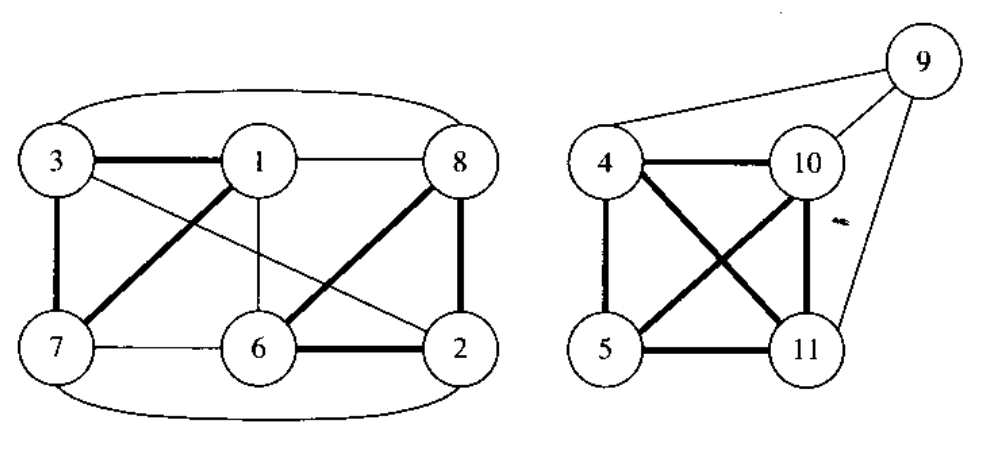
\includegraphics[width=0.5\textwidth]{Compatibility_graph}
    \caption{ Compatibility graph \cite{b1}}
    \label{fig:Compatibility_graph}
\end{figure}
















\subsubsection{Conflict Graph}
$G_{-}(V,E)  $,  is a graph whose vertex set $  V = \{v_{i}, i = 1,2,..., n_{ops}\} $ is in one-to-one correspondence with the operations and whose edge set $ E = \{\{v_{i},v_{j} i,j = 1,2,...,n_{ops}\}$ denotes the conflicting operation pairs \cite{b1}. 

$G_{-}(V,E) $ is the compliment of $G_{+}(V,E)  $ because A set of mutually compatible operations corresponds to a subset of vertices that are not connected by edges, also called the independent set $G_{-}(V,E)  $. A proper vertex coloring of the conflict graph provides a solution to the sharing problem: each color corresponds to a resource instance. An optimum resource sharing corresponds to a vertex coloring with a minimum number of colors. Such a number is the chromatic number of G-(V, E) and is denoted by x(G-(V, E)). Note that 
\begin{center}
$\chi(G_{-}(V,E))  \Leftrightarrow \kappa(G_{+}(V,E)) $
\end{center}

Since operations with different types are always conflicting, it is convenient to consider the conflict graphs for each type independently. Such graphs are the complements of the corresponding compatibility subgraphs for operations of that type. The overall conflict graph can be obtained by adding edges joining any vertex pair with different types to the union of all partial conflict graphs. 

Consider again the scheduled sequencing graph of Figure \ref{Scheduled_sequencing_graph}. We show in Figure \ref{fig:Conflict_graphs_for_the_mtlltiplier_and_ALU_types} the conflict graphs for the multiplier and ALU types. Examples of independent sets are $\{v_{1},v_{3},v_{7}\}  $and$ v_{4},v_{5},v_{10},v_{11} $ among others. Each graph can he colored The clique partitioning and vertex coloring problems have been studied extensively. (See Sections 2.4.4 and 2.4.3.) Both problems are intractable for general graphs, and exact and heuristic solution methods have been proposed. According to the specific circuit type under consideration, the compatibility graph may be sparser than the conflict graph (or vice versa). In this case, clique partitioning (or vertex coloring) may be easier to solve. 

In some particular cases, it is possible to exploit the structure of the sequencing 
graph to derive compatibility and conflict graphs with special properties that make the 
partitioning and coloring tractable. This will be considered in the following section.

$G_{-}(V,E)  $
$\chi(G_{-}(V,E))  $
$\chi(G_{-}(V,E))  \Leftrightarrow \kappa(G_{+}(V,E)) $

\ref{fig:Conflict_graphs_for_the_mtlltiplier_and_ALU_types}
\begin{figure}[h]
    \centering
    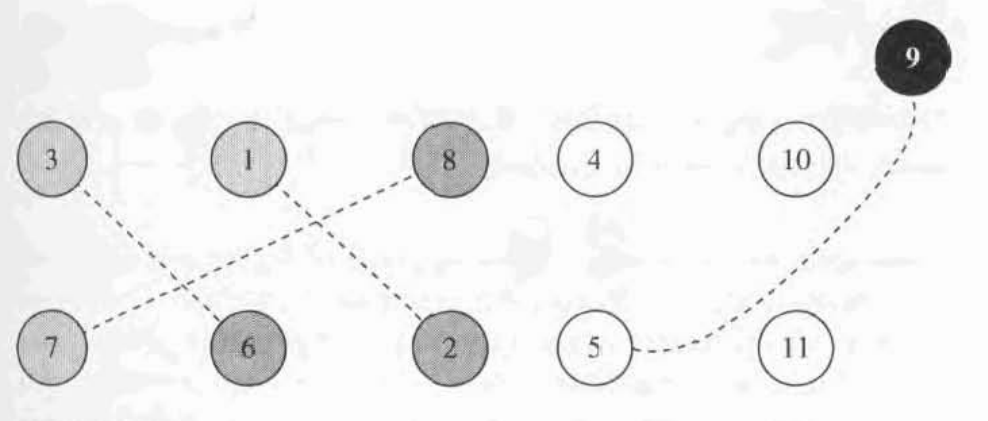
\includegraphics[width=0.5\textwidth]{Conflict_graphs_for_the_mtlltiplier_and_ALU_types}
    \caption{Conflict graphs for the mtlltiplier and ALU types.Conflict graphs for the mtlltiplier and ALU types. \cite{b1}}
    \label{fig:Conflict_graphs_for_the_mtlltiplier_and_ALU_types}
\end{figure}




\subsubsection{Conflict Graph As An Interval}
execution interval $ \{[t_{i},t_{i}+d_{i}-1];i=1,2,...,n_{ops}\} $

\ref{fig:Intervals_corresponding_to_the_conflict_grap}
\begin{figure}[h]
    \centering
    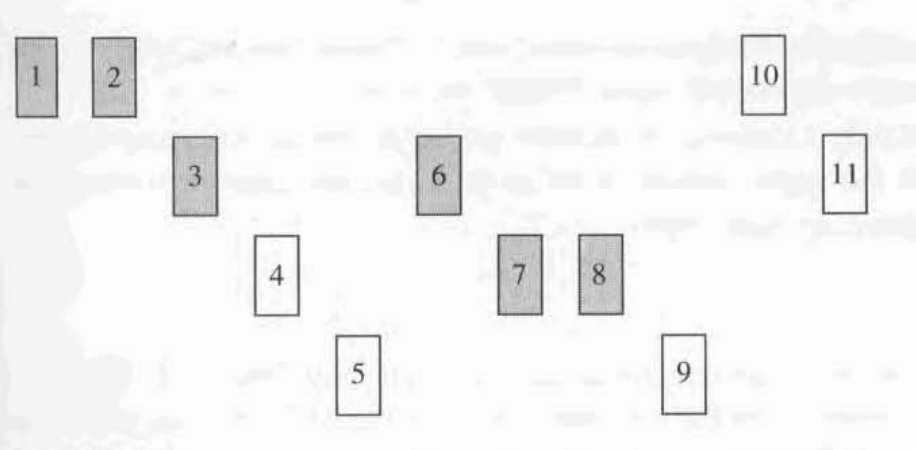
\includegraphics[width=0.5\textwidth]{Intervals_corresponding_to_the_conflict_grap}
    \caption{ Intervals corresponding to the conflict graph \cite{b1}}
    \label{fig:Intervals_corresponding_to_the_conflict_grap}
\end{figure}


\ref{fig:Scheduled_an_bound_sequencing}
\begin{figure}[h]
    \centering
    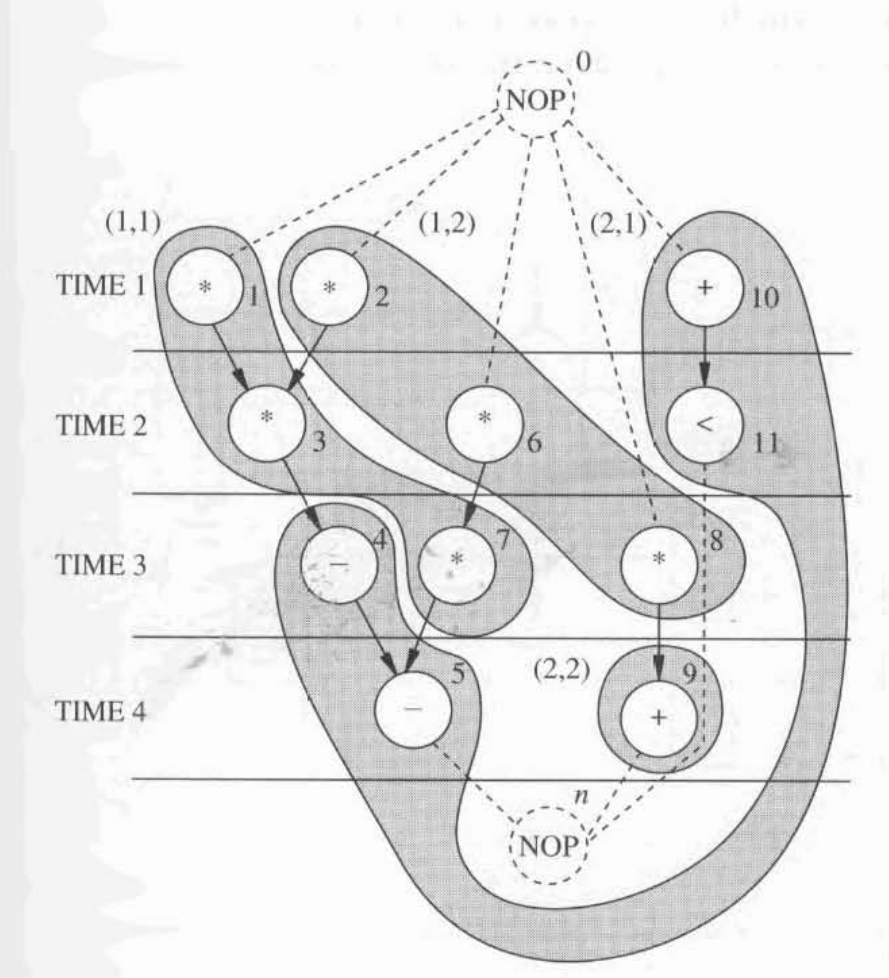
\includegraphics[width=0.5\textwidth]{Scheduled_an_bound_sequencing}
    \caption{ Scheduled and bound sequencing graph \cite{b1}}
    \label{fig:Scheduled_an_bound_sequencing}
\end{figure}










\subsection{Resource sharing and binding in Hierarchical sequence graph}


\subsubsection{Model Call}
\ref{fig:Hierarchical_conflicts_and_compatibility}
\begin{figure}[h]
    \centering
    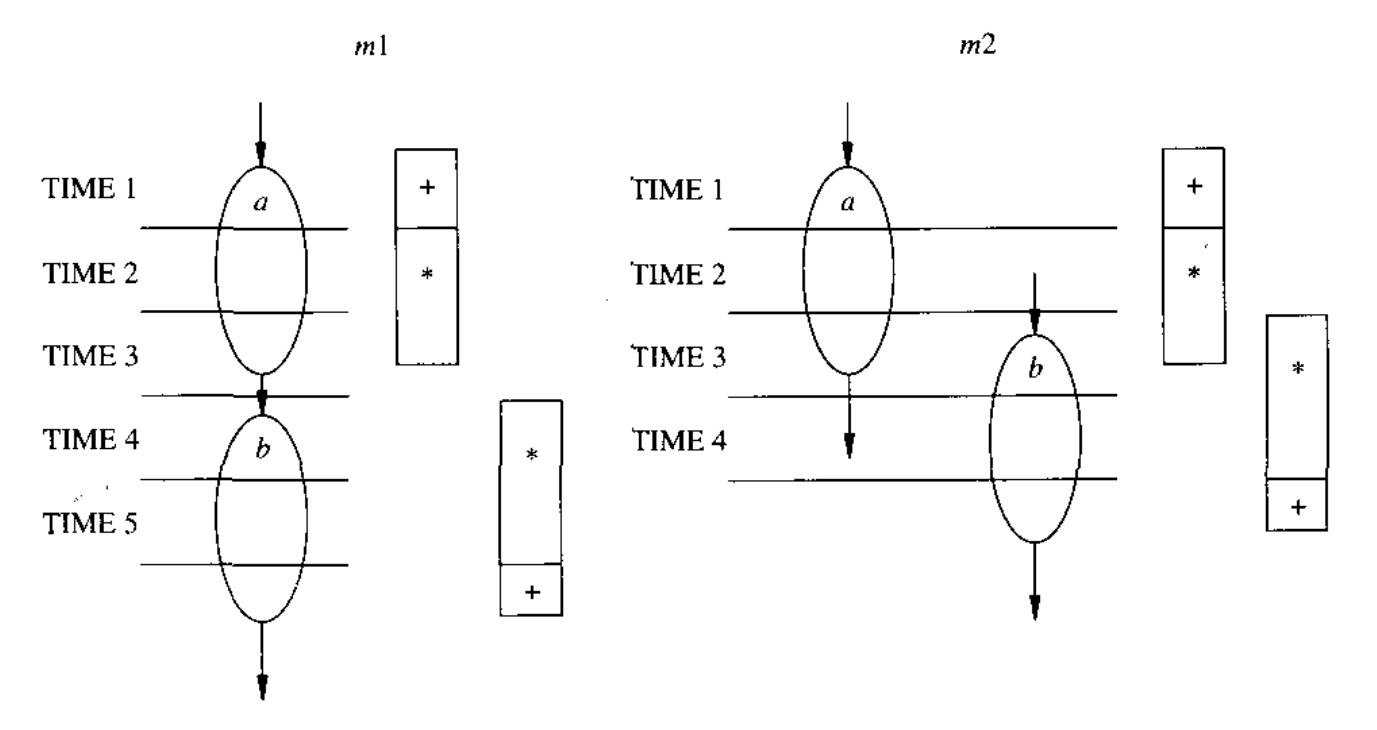
\includegraphics[width=0.5\textwidth]{Hierarchical_conflicts_and_compatibility}
    \caption{ Hierarchical conflicts and compatibility \cite{b1}}
    \label{fig:Hierarchical_conflicts_and_compatibility}
\end{figure}


\begin{itemize}
\item single call
\item multiple call

\ref{fig:Hierarchical_conflicts}
\begin{figure}[h]
    \centering
    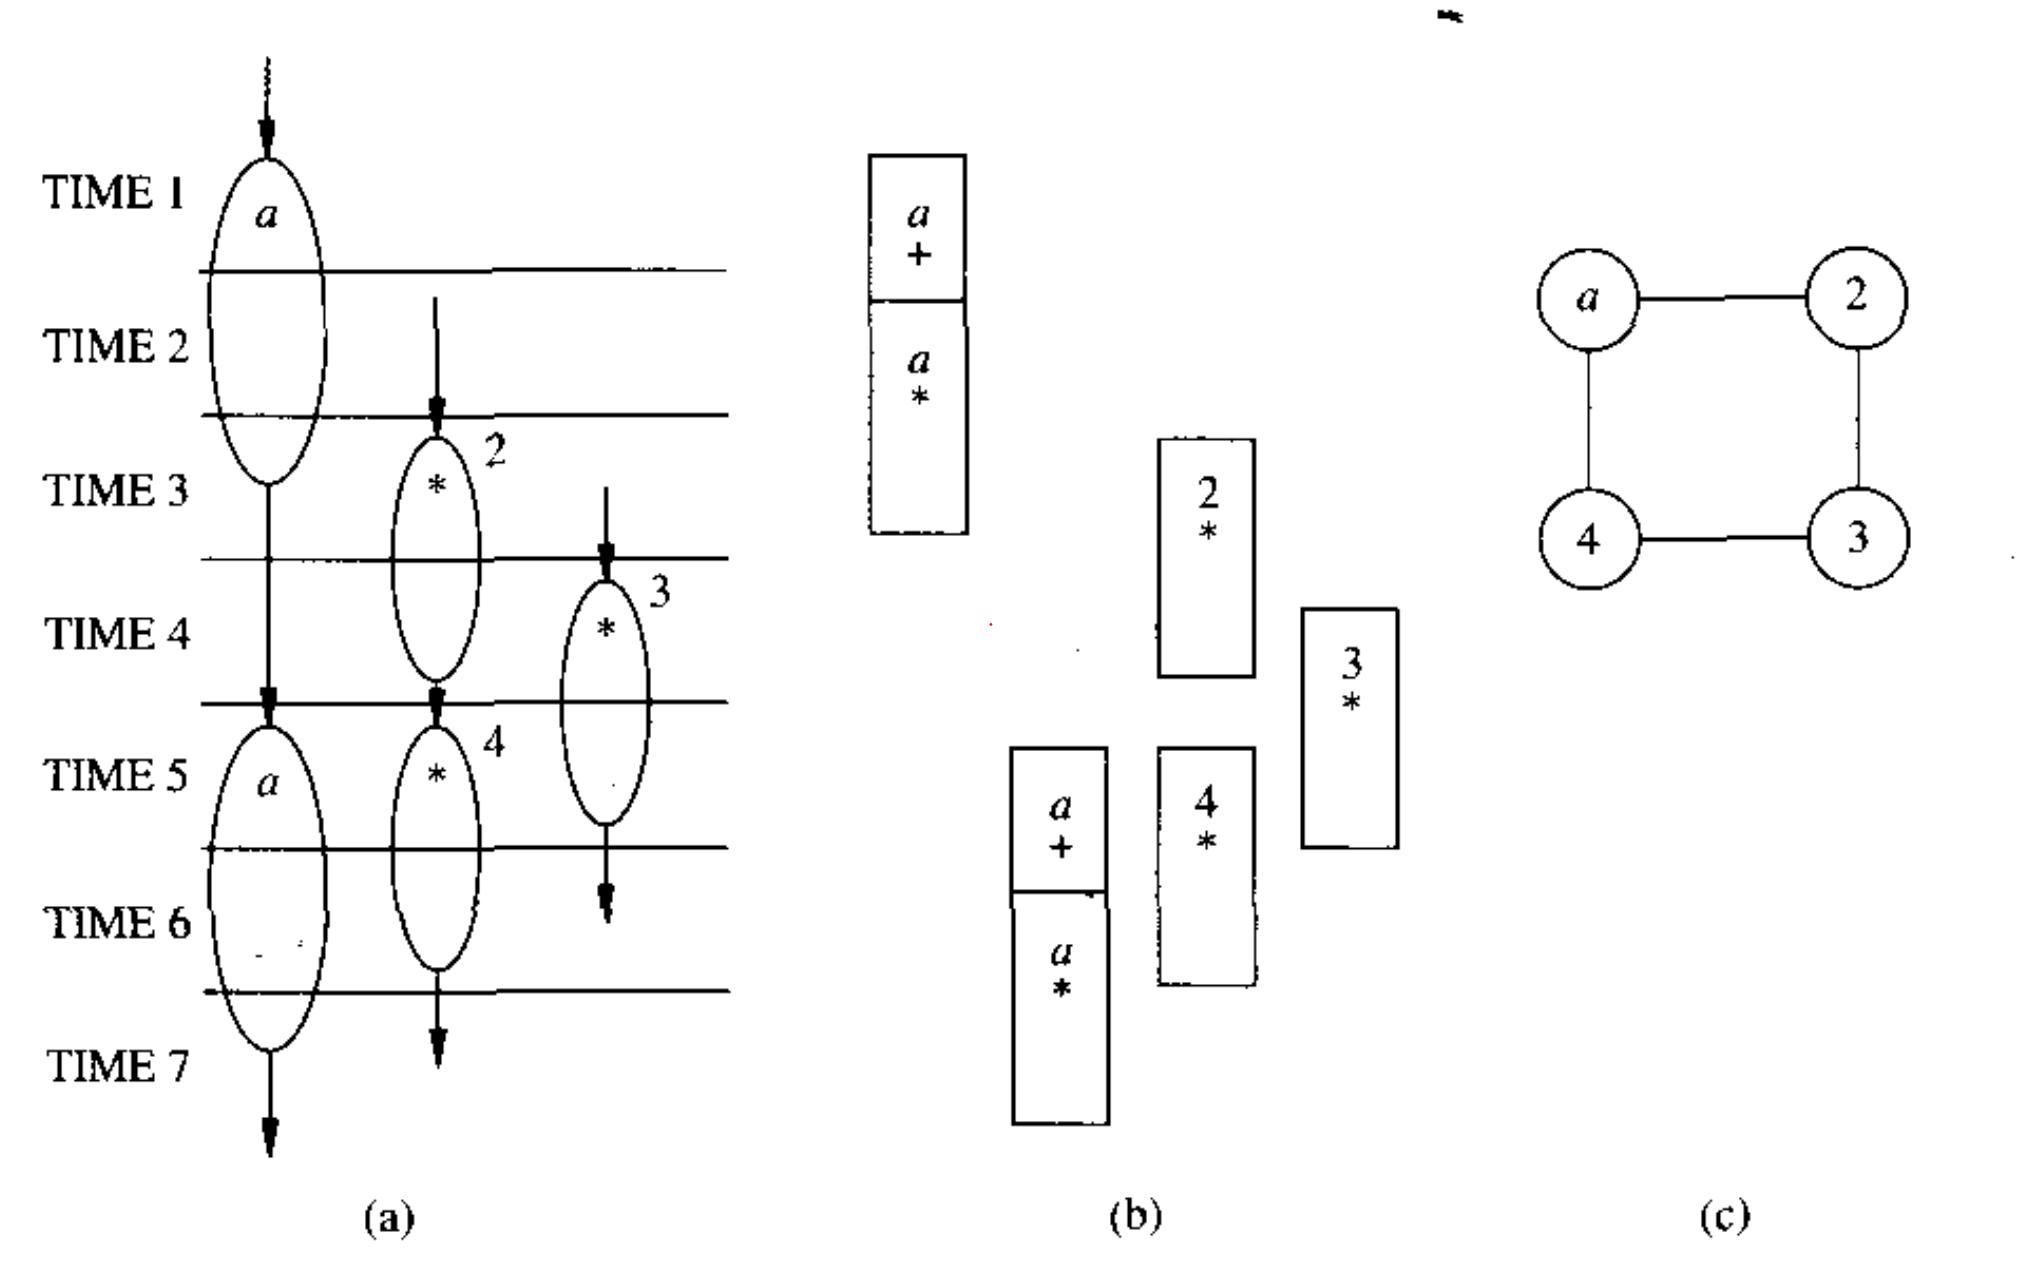
\includegraphics[width=0.5\textwidth]{Hierarchical_conflicts}
    \caption{ Hierarchical conflicts. (a) Sequencing graph fragment. (b) Execution intervals. (c) Non-chordal conflict 
graph \cite{b1}}
    \label{fig:Hierarchical_conflicts}
\end{figure}
\end{itemize}


\subsubsection{Iteration}

\subsubsection{Branching}
\ref{fig:Conditional_execution}
\begin{figure}[h]
    \centering
    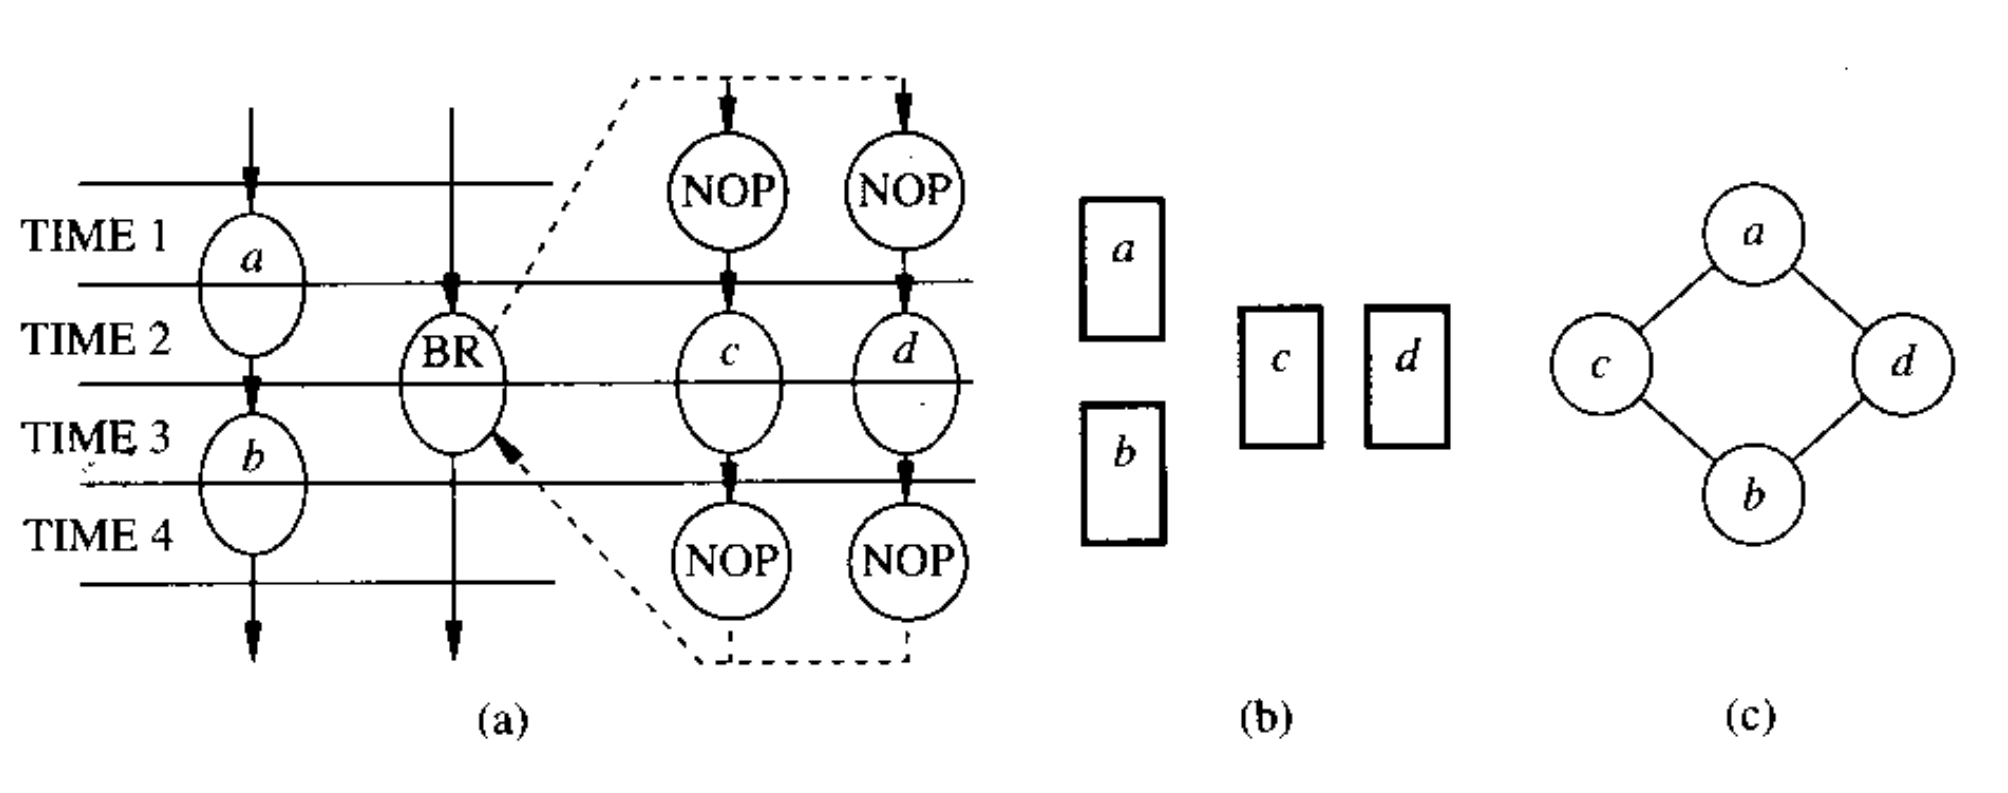
\includegraphics[width=0.5\textwidth]{Conditional_execution}
    \caption{ Conditional execution. (a) Sequencing graph fragment. (b) Execution intervals. (c) Non-chordal conflict 
graph \cite{b1}}
    \label{fig:Conditional_execution}
\end{figure}